\chapter{การ{\wbr}เรียก{\wbr}ตัวเอง: แนว{\wbr}คิด{\wbr}และ{\wbr}พื้นฐาน}

การ{\wbr}เรียก{\wbr}ตัวเอง{\wbr}เป็น{\wbr}แนว{\wbr}คิด{\wbr}ที่{\wbr}ทรง{\wbr}พลัง{\wbr}มาก{\wbr}
เรา{\wbr}จะ{\wbr}ทำ{\wbr}ความ{\wbr}เข้าใจ{\wbr}กับ{\wbr}แนว{\wbr}คิด{\wbr}ดังกล่าว{\wbr}ผ่าน{\wbr}ทาง{\wbr}ตัวอย่าง{\wbr}และ{\wbr}คำถาม{\wbr}
เรา{\wbr}จะ{\wbr}เริ่ม{\wbr}จาก{\wbr}ปัญหา{\wbr}ที่{\wbr}ง่าย{\wbr}และ{\wbr}ตรงไปตรงมา{\wbr}ซึ่ง{\wbr}สามารถ{\wbr}แก้ไข{\wbr}ได้{\wbr}ด้วย{\wbr}อัล{\wbr}กอ{\wbr}ริ{\wbr}ทึม{\wbr}แบบ{\wbr}วน{\wbr}ซ้ำ{\wbr}ทั่วไป{\wbr}
เรา{\wbr}จะ{\wbr}พิจารณา{\wbr}ปัญหา{\wbr}ที่{\wbr}ยาก{\wbr}ขึ้น{\wbr}ใน{\wbr}ตอน{\wbr}ท้าย{\wbr}ของ{\wbr}บท{\wbr}นี้{\wbr}
อย่างไรก็ตาม{\wbr}แนว{\wbr}คิด{\wbr}ของ{\wbr}การ{\wbr}เรียก{\wbr}ตัวเอง{\wbr}จะ{\wbr}เป็น{\wbr}แนว{\wbr}คิด{\wbr}พื้นฐาน{\wbr}ใน{\wbr}การ{\wbr}ทำ{\wbr}ความ{\wbr}เข้าใจ{\wbr}โครงสร้าง{\wbr}ข้อมูล{\wbr}ที่{\wbr}เรา{\wbr}จะ{\wbr}ศึกษา{\wbr}ใน{\wbr}บท{\wbr}อื่น ๆ ด้วย{\wbr}

% TODO: appendix functions
ใน{\wbr}การ{\wbr}ทำ{\wbr}ความ{\wbr}เข้าใจ{\wbr}กับ{\wbr}การ{\wbr}เรียก{\wbr}ตัวเอง{\wbr}นั้น ต้อง{\wbr}ใช้{\wbr}ความ{\wbr}รู้{\wbr}พื้นฐาน{\wbr}เกี่ยวกับ{\wbr}โปรแกรมย่อย{\wbr}
(function ใน{\wbr}ภาษา C++)
ผู้อ่าน{\wbr}สามารถ{\wbr}ทบทวน{\wbr}ได้{\wbr}ที่{\wbr}ภาคผนวก~\ref{appendix:functions}

เรา{\wbr}จะ{\wbr}เริ่ม{\wbr}จาก{\wbr}ปัญหา{\wbr}เกี่ยวกับ{\wbr}การ{\wbr}คำนวณ{\wbr}ที่{\wbr}ข้อมูล{\wbr}ป้อน{\wbr}เข้า{\wbr}เป็น{\wbr}จำนวนเต็ม{\wbr}
จากนั้น{\wbr}จะ{\wbr}พิจารณา{\wbr}ปัญหา{\wbr}ที่{\wbr}ข้อมูล{\wbr}ป้อน{\wbr}เข้า{\wbr}มี{\wbr}ลักษณะ{\wbr}เป็น{\wbr}รายการ เช่น ปัญหา{\wbr}การ{\wbr}หา{\wbr}ค่า{\wbr}มาก{\wbr}ที่สุด{\wbr}
และ{\wbr}ปัญหา{\wbr}การ{\wbr}จัดเรียง{\wbr}ข้อมูล 

\section{การ{\wbr}คำนวณ{\wbr}ทาง{\wbr}พีชคณิต}

เรา{\wbr}จะ{\wbr}เขียน{\wbr}โปรแกรมย่อย{\wbr}ที่{\wbr}บวก{\wbr}จำนวน{\wbr}ธรรมชาติ{\wbr}สอง{\wbr}จำนวน ตัวอย่าง{\wbr}ของ{\wbr}โปรแกรมย่อย{\wbr}นี้{\wbr}แสดง{\wbr}ดัง{\wbr}ด้าน{\wbr}ล่าง{\wbr}

\begin{algt}
\noindent {\bf บวก{\wbr}จำนวน{\wbr}ธรรมชาติ $A$ กับ $B$}\\
\hspace*{0.2in} คำนวณ{\wbr}ค่า $A+B$ แล้ว{\wbr}คืน{\wbr}ผลลัพธ์{\wbr}
\end{algt}

เมื่อ{\wbr}เรา{\wbr}เรียก{\wbr}ใช้{\wbr}โปรแกรมย่อย{\wbr}ดังกล่าว{\wbr}ให้{\wbr}บวก 10 กับ 3 เรา{\wbr}จะ{\wbr}ได้{\wbr}ผลลัพธ์{\wbr}เป็น 13
ลักษณะ{\wbr}ของ{\wbr}การ{\wbr}เรียก{\wbr}ใช้ แสดง{\wbr}ใน{\wbr}รูป~\ref{rec:add-call}

\begin{figure}
\begin{center}
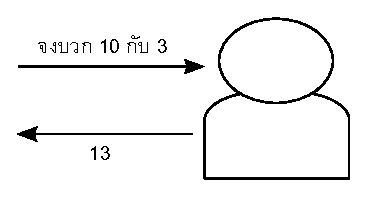
\epsfig{file=figures/recursion/add-call.eps, height=1in}
\end{center}
\caption{ตัวอย่าง{\wbr}การ{\wbr}เรียก{\wbr}ใช้{\wbr}โปรแกรมย่อย}
\label{rec:add-call}
\end{figure}

เรา{\wbr}จะ{\wbr}ปรับ{\wbr}โปรแกรมย่อย{\wbr}ดังกล่าว ให้{\wbr}เป็น{\wbr}โปรแกรมย่อย{\wbr}แบบ{\wbr}เรียก{\wbr}ตัวเอง{\wbr}
สมมติ{\wbr}ว่า{\wbr}เรา{\wbr}ทราบ{\wbr}วิธีการ{\wbr}เพิ่ม{\wbr}ค่า{\wbr}จำนวน{\wbr}ธรรมชาติ{\wbr}ขึ้น 1 และ{\wbr}ลด{\wbr}ค่า{\wbr}จำนวน{\wbr}ธรรมชาติ{\wbr}ลง 1
พิจารณา{\wbr}วิธีการ{\wbr}บวก{\wbr}จำนวน{\wbr}ธรรมชาติ $A$ เข้า{\wbr}กับ $B$
ดัง{\wbr}อัล{\wbr}กอ{\wbr}ริ{\wbr}ทึม{\wbr}ที่~\ref{algo:rec-int-add}

\begin{figure}
\begin{algt}
\label{algo:rec-int-add}
\noindent {\bf บวก{\wbr}จำนวน{\wbr}ธรรมชาติ $A$ กับ $B$}\\
\hspace*{0.2in} IF $B=0$ THEN RETURN $A$\\
\hspace*{0.2in} ELSE\\
\hspace*{0.2in}\hspace*{0.2in} LET $C\leftarrow B-1$\\
\hspace*{0.2in}\hspace*{0.2in} ให้ $D$ เท่า{\wbr}กับ{\wbr}ผลบวก{\wbr}ของ $A$ กับ $C$\\
\hspace*{0.2in}\hspace*{0.2in} RETURN $D+1$
\end{algt}
\end{figure}

นิยาม{\wbr}ข้างต้น{\wbr}มี{\wbr}ลักษณะ{\wbr}เหมือน{\wbr}งู{\wbr}กิน{\wbr}หาง{\wbr}
เพราะว่า{\wbr}เรา{\wbr}กำลัง{\wbr}นิยาม{\wbr}การ{\wbr}บวก{\wbr}จำนวน{\wbr}ธรรมชาติ{\wbr}ด้วย{\wbr}การ{\wbr}บวก{\wbr}จำนวน{\wbr}ธรรมชาติ อย่างไรก็ตาม{\wbr}
เรา{\wbr}จะ{\wbr}ละ{\wbr}ความ{\wbr}สงสัย{\wbr}ดังกล่าว{\wbr}ไว้{\wbr}ก่อน{\wbr}แล้ว{\wbr}ทดลอง{\wbr}บวก 10 กับ 3 ดังนี้{\wbr}

\begin{itemize}
\item เนื่องจาก $3$ ไม่{\wbr}เท่า{\wbr}กับ $0$ เรา{\wbr}จึง{\wbr}คำนวณ{\wbr}ค่า $3-1 = 2$
จากนั้น{\wbr}เรา{\wbr}ต้องการ{\wbr}คำนวณ{\wbr}หา{\wbr}ผลบวก{\wbr}ของ $10$ กับ $2$ เมื่อ{\wbr}ได้{\wbr}ผลบวก{\wbr}แล้ว เรา{\wbr}จะ{\wbr}เพิ่ม{\wbr}ค่า{\wbr}ขึ้น{\wbr}
$1$ เพื่อ{\wbr}ได้{\wbr}ผลบวก{\wbr}ของ $10$ กับ $3$ ตาม{\wbr}ต้องการ{\wbr}
\end{itemize}

\begin{figure}
\begin{center}
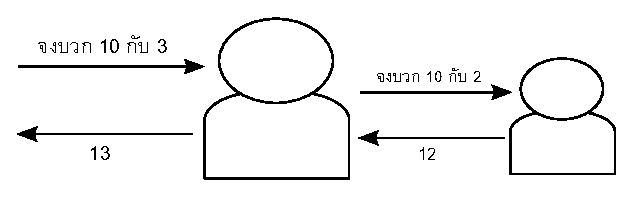
\epsfig{file=figures/recursion/add-2-calls.eps, height=1in}
\end{center}
\caption{ตัวอย่าง{\wbr}การ{\wbr}เรียก{\wbr}ใช้{\wbr}โปรแกรมย่อย{\wbr}ที่{\wbr}เรียก{\wbr}ใช้{\wbr}โปรแกรมย่อย{\wbr}เพื่อ{\wbr}คำนวณ{\wbr}ผลบวก{\wbr}ของ 10 กับ 2}
\label{rec:add-2-calls}
\end{figure}


จาก{\wbr}ขั้นตอน{\wbr}ด้าน{\wbr}บน ถ้า{\wbr}เรา{\wbr}ทราบ{\wbr}ว่า{\wbr}ผลบวก{\wbr}ของ $10$ กับ $2$ คือ $12$ เมื่อ{\wbr}เพิ่ม{\wbr}ค่า{\wbr}ขึ้น $1$
เรา{\wbr}จะ{\wbr}ได้{\wbr}ผลลัพธ์{\wbr}ของ $10$ กับ $3$ ซึ่ง{\wbr}มี{\wbr}ค่า{\wbr}เท่า{\wbr}กับ $13$ \ \ \
รูป~\ref{rec:add-2-calls} แสดง{\wbr}การ{\wbr}ทำงาน{\wbr}ของ{\wbr}โปรแกรมย่อย{\wbr}ดังกล่าว{\wbr}


\begin{quiz}{10 + 2}
เรา{\wbr}จะ{\wbr}หา{\wbr}ผลลัพธ์{\wbr}ของ{\wbr}การ{\wbr}บวก $10$ กับ $2$ ได้{\wbr}อย่างไร?
\end{quiz}

เรา{\wbr}ก็{\wbr}จะ{\wbr}หา{\wbr}ผลลัพธ์{\wbr}ด้วย{\wbr}วิธี{\wbr}เดียวกัน ซึ่ง{\wbr}ใน{\wbr}การ{\wbr}ผลบวก เรา{\wbr}จะ{\wbr}ต้องหา{\wbr}ผลลัพธ์{\wbr}ของ{\wbr}การ{\wbr}บวก $10$ กับ{\wbr}
$1$ และ{\wbr}จะ{\wbr}เป็น{\wbr}เช่นนี้{\wbr}เป็น{\wbr}เรื่อย ๆ ดัง{\wbr}ตัวอย่าง{\wbr}ด้าน{\wbr}ล่าง (รูป{\wbr}ที่~\ref{rec:add-rec-calls}
แสดง{\wbr}ลักษณะ{\wbr}การ{\wbr}คำนวณ)


\begin{itemize}
\item เนื่องจาก $3$ ไม่{\wbr}เท่า{\wbr}กับ $0$ เรา{\wbr}จึง{\wbr}คำนวณ{\wbr}ค่า $3-1 = 2$ จากนั้น{\wbr}เรา{\wbr}ต้องการ{\wbr}คำนวณ{\wbr}หา{\wbr}ผลบวก{\wbr}ของ $10$ กับ $2$ ใน{\wbr}การ{\wbr}คำนวณ{\wbr}ผลบวก{\wbr}ดังกล่าว เรา{\wbr}จะ{\wbr}ใช้{\wbr}วิธีการ{\wbr}เดิม{\wbr}
\begin{itemize}
\item เนื่องจาก $2$ ไม่{\wbr}เท่า{\wbr}กับ $0$ เรา{\wbr}จึง{\wbr}คำนวณ{\wbr}ค่า $2-1 = 1$ จากนั้น{\wbr}เรา{\wbr}ต้องการ{\wbr}คำนวณ{\wbr}หา{\wbr}ผลบวก{\wbr}ของ $10$ กับ $1$ ใน{\wbr}การ{\wbr}คำนวณ{\wbr}ผลบวก{\wbr}ดังกล่าว เรา{\wbr}จะ{\wbr}ใช้{\wbr}วิธีการ{\wbr}เดิม{\wbr}
\begin{itemize}
\item เนื่องจาก $1$ ไม่{\wbr}เท่า{\wbr}กับ $0$ เรา{\wbr}จึง{\wbr}คำนวณ{\wbr}ค่า $1-1 = 0$ จากนั้น{\wbr}เรา{\wbr}ต้องการ{\wbr}คำนวณ{\wbr}หา{\wbr}ผลบวก{\wbr}ของ $10$ กับ $0$ ใน{\wbr}การ{\wbr}คำนวณ{\wbr}ผลบวก{\wbr}ดังกล่าว เรา{\wbr}จะ{\wbr}ใช้{\wbr}วิธีการ{\wbr}เดิม{\wbr}
\begin{itemize}
\item เนื่องจาก $0$ เท่า{\wbr}กับ $0$ ผลลัพธ์{\wbr}ของ{\wbr}การ{\wbr}บวก $10$ กับ $0$ คือ $10$
\end{itemize}
\item เมื่อ{\wbr}เรา{\wbr}ได้{\wbr}ผลลัพธ์{\wbr}ของ{\wbr}การ{\wbr}บวก $10$ กับ $0$ แล้ว (คือ $10$) เรา{\wbr}คำนวณ $10+1$ ได้{\wbr}ผลลัพธ์ $11$ ซึ่ง{\wbr}เป็น{\wbr}ผลลัพธ์{\wbr}ของ{\wbr}การ{\wbr}บวก $10$ กับ $1$
\end{itemize}
\item เมื่อ{\wbr}เรา{\wbr}ได้{\wbr}ผลลัพธ์{\wbr}ของ{\wbr}การ{\wbr}บวก $10$ กับ $1$ แล้ว (คือ $11$) เรา{\wbr}คำนวณ $11+1$ ได้{\wbr}ผลลัพธ์ $12$ ซึ่ง{\wbr}เป็น{\wbr}ผลลัพธ์{\wbr}ของ{\wbr}การ{\wbr}บวก $10$ กับ $2$
\end{itemize}
\item เมื่อ{\wbr}เรา{\wbr}ได้{\wbr}ผลลัพธ์{\wbr}ของ{\wbr}การ{\wbr}บวก $10$ กับ $2$ แล้ว (คือ $12$) เรา{\wbr}คำนวณ $12+1$ ได้{\wbr}ผลลัพธ์ $13$ ซึ่ง{\wbr}เป็น{\wbr}ผลลัพธ์{\wbr}ของ{\wbr}การ{\wbr}บวก $10$ กับ $3$
\end{itemize}


\begin{figure}
\begin{center}
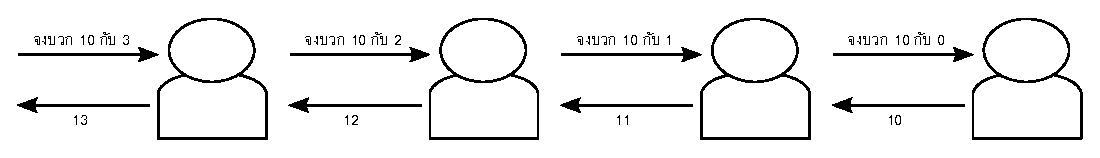
\epsfig{file=figures/recursion/add-rec-calls.eps, width=6in}
\end{center}
\caption{ตัวอย่าง{\wbr}การ{\wbr}เรียก{\wbr}ใช้{\wbr}โปรแกรมย่อย{\wbr}ที่{\wbr}เรียก{\wbr}ตัวเอง}
\label{rec:add-rec-calls}
\end{figure}


\begin{quiz}{การ{\wbr}ลบ}
เขียน{\wbr}ขั้นตอน{\wbr}การ{\wbr}ลบ{\wbr}จำนวน{\wbr}ธรรมชาติ $A$ กับ $B$ ใน{\wbr}รูปแบบ{\wbr}เดียวกับ{\wbr}การ{\wbr}คำนวณ{\wbr}ผลบวก{\wbr}
\end{quiz}

\begin{quiz}{การ{\wbr}คูณ}
เขียน{\wbr}ขั้นตอน{\wbr}การ{\wbr}คูณ{\wbr}จำนวน{\wbr}ธรรมชาติ $A$ กับ $B$ ใน{\wbr}รูปแบบ{\wbr}เดียวกับ{\wbr}การ{\wbr}คำนวณ{\wbr}ผลบวก{\wbr}
\end{quiz}

\begin{quiz}{ศูนย์}
ถ้า{\wbr}เรา{\wbr}ตัด{\wbr}บรรทัด{\wbr}แรก{\wbr}ที่{\wbr}ระบุ{\wbr}เงื่อนไข{\wbr}ที่ทำงาน{\wbr}เมื่อ $B=0$ ออก  เมื่อ{\wbr}เรา{\wbr}ดำเนินการ{\wbr}ตาม{\wbr}ขั้นตอนวิธี{\wbr}ดังกล่าว ผลลัพธ์{\wbr}จะ{\wbr}เป็น{\wbr}เช่น{\wbr}ใด{\wbr}
\end{quiz}

เรา{\wbr}สามารถ{\wbr}เขียน{\wbr}อัล{\wbr}กอ{\wbr}ริ{\wbr}ทึม{\wbr}ดังกล่าว{\wbr}เป็น{\wbr}โปรแกรม{\wbr}ได้{\wbr}ไม่{\wbr}ยาก{\wbr}ดังนี้{\wbr}

\latintext
\begin{codelist}{C++}{}
int add(int a, int b)
{
  if(b==0)
    return a;

  int c = b-1;
  return 1 + add(a,c);
}
\end{codelist}
\thaitext

\section{ค่าสูงสุด}

เรา{\wbr}จะ{\wbr}ออกแบบ{\wbr}อัล{\wbr}กอ{\wbr}ริ{\wbr}ทึม{\wbr}แบบ{\wbr}เรียก{\wbr}ตัวเอง{\wbr}สำหรับ{\wbr}การ{\wbr}คำนวณ{\wbr}ค่าสูงสุด กล่าวคือ{\wbr}
ให้{\wbr}อาร์เรย์ $A$ ของ{\wbr}จำนวนเต็ม $n$ จำนวน เรา{\wbr}ต้องการ{\wbr}คำนวณ{\wbr}ค่าสูงสุด{\wbr}

กรณี{\wbr}ที่{\wbr}เรา{\wbr}สามารถ{\wbr}ตอบ{\wbr}คำถาม{\wbr}ได้{\wbr}ง่าย คือ{\wbr}กรณี{\wbr}ที่ $n=1$
กล่าวคือ{\wbr}เรา{\wbr}สามารถ{\wbr}ตอบ{\wbr}ได้{\wbr}ทันที{\wbr}ว่า{\wbr}ค่าสูงสุด{\wbr}เท่า{\wbr}กับ $A[0]$

\begin{algt}
\noindent {\bf การ{\wbr}คำ{\wbr}น{\wbr}วน{\wbr}ค่าสูงสุด{\wbr}ของ{\wbr}อาร์เรย์ $A$ ที่{\wbr}มี{\wbr}สมาชิก $n$ ตัว (ขั้น{\wbr}ฐาน)}\\
\hspace*{0.2in} IF $n=1$ THEN RETURN $A[0]$\\
\hspace*{0.2in} ELSE\\
\hspace*{0.2in}\hspace*{0.2in} {\em จะ{\wbr}ต้อง{\wbr}ออกแบบ{\wbr}ต่อไป}
\end{algt}

สำหรับ{\wbr}บท{\wbr}นี้{\wbr}เพื่อ{\wbr}ความ{\wbr}สะดวก{\wbr}ใน{\wbr}การ{\wbr}เขียน{\wbr}
แทน{\wbr}ที่{\wbr}เรา{\wbr}จะ{\wbr}เรียก{\wbr}ข้อมูล{\wbr}ใน{\wbr}อาร์เรย์{\wbr}โดย{\wbr}เขียน{\wbr}ใน{\wbr}วงเล็บ{\wbr}เหลี่ยม เช่น $A[4]$ หรือ $A[i]$
เรา{\wbr}จะ{\wbr}เขียน{\wbr}เป็น{\wbr}ตัว{\wbr}ห้อย เช่น $A_4$ หรือ $A_i$
และ{\wbr}จะ{\wbr}เขียน{\wbr}อาร์เรย์{\wbr}โดย{\wbr}ระบุ{\wbr}ข้อมูล{\wbr}ใน{\wbr}อาร์เรย์{\wbr}ใน{\wbr}วงเล็บ{\wbr}เหลี่ยม เช่น อาร์เรย์
$[2,3,5,7,11]$ เป็นต้น{\wbr}

สำหรับ{\wbr}กรณี{\wbr}ทั่วไป เรา{\wbr}จะ{\wbr}เริ่ม{\wbr}โดย{\wbr}พิจารณา{\wbr}ปัญหา{\wbr}เมื่อ{\wbr}ข้อมูล{\wbr}นำเข้า{\wbr}มี{\wbr}ขนาด{\wbr}เล็ก{\wbr}ลง โดย{\wbr}เรา{\wbr}จะ{\wbr}ให้{\wbr}
\[
A' = [A_0,A_1,\ldots,A_{n-2}]
\]
นั่น{\wbr}คือ $A'$ คือ{\wbr}อาร์เรย์ $A$ ที่{\wbr}ตัด{\wbr}ข้อมูล{\wbr}ตัว{\wbr}สุดท้าย{\wbr}ทิ้ง{\wbr}ไป{\wbr}

ปัญหา{\wbr}นี้{\wbr}เรา{\wbr}จะ{\wbr}เรียก{\wbr}ว่า {\em ปัญหา{\wbr}ย่อย} (subproblem)
เรา{\wbr}จะ{\wbr}สมมติ{\wbr}ว่า{\wbr}เรา{\wbr}สามารถ{\wbr}หา{\wbr}คำตอบ{\wbr}ของ{\wbr}ปัญหา{\wbr}ได้ กล่าวคือ{\wbr}
ให้ $M$ คือ{\wbr}ค่าสูงสุด{\wbr}ของ{\wbr}อาร์เรย์ $A'$

\begin{quiz}{ค่า{\wbr}สูง{\wbr}ที่สุด{\wbr}จาก $M$}
สมมติ{\wbr}ว่า{\wbr}เรา{\wbr}ทราบ{\wbr}ว่า $M$ คือ{\wbr}ค่าสูงสุด{\wbr}ของ{\wbr}อาร์เรย์ $A'= [A_0,A_1,\ldots,A_{n-2}]$
เรา{\wbr}สามารถ{\wbr}คำนวณ{\wbr}ค่าสูงสุด{\wbr}ของ{\wbr}อาร์เรย์ 
$A= [A_0,A_1,\ldots,A_{n-1}]$
ได้{\wbr}อย่างไร?

(คำ{\wbr}ใบ้: ถ้า $M$ ไม่{\wbr}ใช่{\wbr}ข้อมูล{\wbr}ที่{\wbr}มี{\wbr}ค่าสูงสุด{\wbr}ของ{\wbr}อาร์เรย์ ค่า{\wbr}อื่น{\wbr}ที่{\wbr}เป็น{\wbr}ไป{\wbr}ได้{\wbr}คือ{\wbr}ค่า{\wbr}ใด?)
\end{quiz}

เมื่อ{\wbr}เรา{\wbr}พิจารณา{\wbr}ข้อมูล{\wbr}สูงสุด{\wbr}ของ{\wbr}อาร์เรย์ $A$ มี{\wbr}ความ{\wbr}เป็น{\wbr}ไป{\wbr}ได้{\wbr}สอง{\wbr}กรณี{\wbr}คือ{\wbr}
กรณี{\wbr}ที่{\wbr}ข้อมูล{\wbr}สูง{\wbr}ที่สุด{\wbr}อยู่{\wbr}ใน{\wbr}อาร์เรย์ $A'$ ใน{\wbr}อีก{\wbr}กรณี{\wbr}หนึ่ง{\wbr}คือ{\wbr}ข้อมูล{\wbr}สูง{\wbr}ที่สุด{\wbr}คือ $x_n$
ถ้า{\wbr}เป็น{\wbr}ใน{\wbr}กรณี{\wbr}แรก{\wbr}ค่าสูงสุด{\wbr}คือ $M$ ใน{\wbr}อีก{\wbr}กรณี{\wbr}หนึ่ง{\wbr}คือ ข้อมูล{\wbr}ตัว{\wbr}สุดท้าย $A_{n-1}$ ใน $A$
ซึ่ง{\wbr}เรา{\wbr}สามารถ{\wbr}เทียบ{\wbr}ข้อมูล{\wbr}ทั้ง{\wbr}สอง{\wbr}เพื่อ{\wbr}หา{\wbr}ค่า{\wbr}สูง{\wbr}ที่สุด{\wbr}ได้ ดัง{\wbr}อัล{\wbr}กอ{\wbr}ริ{\wbr}ทึม{\wbr}ด้าน{\wbr}ล่าง{\wbr}

\begin{algt}
\label{}
\noindent {\bf การ{\wbr}คำ{\wbr}น{\wbr}วน{\wbr}ค่าสูงสุด{\wbr}ของ{\wbr}อาร์เรย์ $A$ ที่{\wbr}มี{\wbr}สมาชิก $n$ ตัว}\\
1.\settowidth{\algbackindent}{1.}\hspace*{-\algbackindent}\hspace*{0.2in} IF $n=1$ THEN RETURN $A[0]$\\
2.\settowidth{\algbackindent}{2.}\hspace*{-\algbackindent}\hspace*{0.2in} ELSE\\
3.\settowidth{\algbackindent}{3.}\hspace*{-\algbackindent}\hspace*{0.2in}\hspace*{0.2in} ให้ $M$ คือ{\wbr}ค่าสูงสุด{\wbr}ของ{\wbr}อาร์เรย์ $A'$ ที่{\wbr}มี{\wbr}สมาชิก $n-1$ ตัว เมื่อ $A' = [A_0,A_1,\ldots,A_{n-2}]$\\
4.\settowidth{\algbackindent}{4.}\hspace*{-\algbackindent}\hspace*{0.2in}\hspace*{0.2in} IF $A_{n-1} > M$ THEN \\
5.\settowidth{\algbackindent}{5.}\hspace*{-\algbackindent}\hspace*{0.2in}\hspace*{0.2in}\hspace*{0.2in} RETURN $A_{n-1}$\\
6.\settowidth{\algbackindent}{6.}\hspace*{-\algbackindent}\hspace*{0.2in}\hspace*{0.2in} ELSE\\
7.\settowidth{\algbackindent}{7.}\hspace*{-\algbackindent}\hspace*{0.2in}\hspace*{0.2in}\hspace*{0.2in} RETURN $M$
\end{algt}

คำถาม{\wbr}ก็{\wbr}คือ ใน{\wbr}ขั้นตอน{\wbr}ที่ 3 เรา{\wbr}จะ{\wbr}คำนวณ{\wbr}หา{\wbr}ค่า $M$ ได้{\wbr}อย่างไร?
สังเกต{\wbr}ว่า{\wbr}ปัญหา{\wbr}ดังกล่าว{\wbr}ก็{\wbr}คือ{\wbr}ปัญหา{\wbr}เดียวกับ{\wbr}ปัญหา{\wbr}เริ่มต้น{\wbr}ที่{\wbr}เรา{\wbr}ต้องการ{\wbr}จะ{\wbr}แก้{\wbr}
แต่{\wbr}มี{\wbr}ข้อมูล{\wbr}ป้อน{\wbr}เข้าที่{\wbr}แตกต่าง{\wbr}ออก{\wbr}ไป ดังนั้น ใน{\wbr}การ{\wbr}แก้{\wbr}ปัญหา{\wbr}ดังกล่าว{\wbr}
เรา{\wbr}ก็{\wbr}จะ{\wbr}เรียก{\wbr}ฟังก์ชัน{\wbr}ที่{\wbr}เรา{\wbr}เตรียม{\wbr}ไว้{\wbr}สำหรับ{\wbr}แก้{\wbr}ปัญหา{\wbr}นั้น นั่น{\wbr}ก็{\wbr}คือ{\wbr}ฟังก์ชัน{\wbr}ที่{\wbr}เรา{\wbr}กำลัง{\wbr}เขียน{\wbr}อยู่{\wbr}นั่นเอง{\wbr}

จาก{\wbr}แนว{\wbr}คิด{\wbr}ดังกล่าว เรา{\wbr}สามารถ{\wbr}พัฒนา{\wbr}โปรแกรม{\wbr}ที่{\wbr}คำนวณ{\wbr}ค่าสูงสุด{\wbr}ได้{\wbr}ดังนี้{\wbr}

\latintext
\begin{codelist}{C++}{}
int arraymax(int ar[], int n)
{
  if(n==1)
    return ar[0];
  else {
    int m = arraymax(ar,n-1);   // Line 6
    if(m > xn)
      return m;
    else
      return ar[n-1];
  }
}
\end{codelist}
\thaitext

สังเกต{\wbr}ว่า{\wbr}ใน{\wbr}โปรแกรม{\wbr}ดังกล่าว เรา{\wbr}ไม่{\wbr}ได้{\wbr}สร้าง{\wbr}อาร์เรย์ $A'$ ขึ้น{\wbr}มา{\wbr}ใหม่{\wbr}แต่อย่างใด{\wbr}
เนื่องจาก{\wbr}วิธีการ{\wbr}เรา{\wbr}สามารถ{\wbr}พิจารณา{\wbr}ให้ $A'$ เป็น{\wbr}แค่{\wbr}ส่วน{\wbr}ต้น{\wbr}ของ{\wbr}อาร์เรย์ $A$
สิ่ง{\wbr}ที่{\wbr}เรา{\wbr}ทำ{\wbr}เพื่อ{\wbr}ป้อน{\wbr}เป็น{\wbr}ข้อมูล{\wbr}ป้อน{\wbr}เข้า{\wbr}ให้{\wbr}กับ{\wbr}ฟังก์ชัน {\ct arraymax}
คือ{\wbr}ปรับ{\wbr}จำนวน{\wbr}ของ{\wbr}ข้อมูล{\wbr}ใน{\wbr}อาร์เรย์{\wbr}เท่านั้น{\wbr}เอง{\wbr}

\begin{quiz}{ผลบวก{\wbr}ของ{\wbr}อาร์เรย์}
ออกแบบ{\wbr}อัล{\wbr}กอ{\wbr}ริ{\wbr}ทึม{\wbr}ที่{\wbr}รับ{\wbr}อาร์เรย์ $A$ ของ{\wbr}จำนวนเต็ม $n$ จำนวน{\wbr}
แล้ว{\wbr}คำนวณ{\wbr}ผลรวม{\wbr}ของ{\wbr}ข้อมูล{\wbr}ใน{\wbr}รายการ{\wbr}
\end{quiz}

\begin{quiz}{เปลี่ยน{\wbr}ทิศทาง}
แทน{\wbr}ที่{\wbr}เรา{\wbr}จะ{\wbr}นิยาม{\wbr}ให้ $A'$ เป็น{\wbr}อาร์เรย์ $A$ ที่{\wbr}ลบ{\wbr}ข้อมูล{\wbr}ตัว{\wbr}สุดท้าย{\wbr}ออก{\wbr}ไป เรา{\wbr}อาจ{\wbr}จะ{\wbr}นิยาม{\wbr}
\[
A'=[A_1,A_2,\ldots,A_{n-1}]
\]
นั่น{\wbr}คือ ให้{\wbr}เป็น{\wbr}อาร์เรย์ $A$ ที่{\wbr}ลบ{\wbr}ข้อมูล{\wbr}ตัว{\wbr}แรก{\wbr}ออก{\wbr}
จง{\wbr}พัฒนา{\wbr}อัล{\wbr}กอ{\wbr}ริ{\wbr}ทึม{\wbr}หา{\wbr}ค่า{\wbr}มาก{\wbr}ที่สุด{\wbr}โดย{\wbr}ใช้{\wbr}การ{\wbr}เรียก{\wbr}ตัวเอง{\wbr}บน{\wbr}อาร์เรย์ $A'$ ที่{\wbr}นิยาม{\wbr}ใหม่{\wbr}นี้{\wbr}
และ{\wbr}เขียน{\wbr}โปรแกรม{\wbr}

(คำแนะนำ{\wbr}เพิ่มเติม: ใน{\wbr}การ{\wbr}ส่ง{\wbr}ค่า $A'$ ใน{\wbr}การ{\wbr}เรียก{\wbr}ตัวเอง{\wbr}อาจ{\wbr}จะ{\wbr}ดู{\wbr}ซับซ้อน{\wbr}กว่า{\wbr}วิธี{\wbr}เก่า{\wbr}เล็กน้อย{\wbr}
แต่{\wbr}อย่า{\wbr}ลืม{\wbr}ว่า{\wbr}เรา{\wbr}สามารถ{\wbr}บวก{\wbr}พอยน์เตอร์{\wbr}ได้)
\end{quiz}



\subsection{ฟังก์ชัน{\wbr}เรียก{\wbr}ตัวเอง}
อัล{\wbr}กอ{\wbr}ริ{\wbr}ทึม{\wbr}ดังกล่าว{\wbr}สามารถ{\wbr}พิจารณา{\wbr}ว่า{\wbr}เป็น{\wbr}การ{\wbr}คำนวณ{\wbr}ค่า{\wbr}ฟังก์ชัน $f$ ที่{\wbr}มี{\wbr}นิยาม{\wbr}ดังต่อไปนี้{\wbr}

$f([A_0,A_1,\ldots,A_{n-1}]) = 
\left\{
\begin{array}{ll}
A_0, &  \mbox{ถ้า } n=1 \\
\max \{ A_{n-1},f([A_0,A_1,\ldots,A_{n-2}]) \},  & \mbox{ใน{\wbr}กรณี{\wbr}อื่น ๆ}
\end{array}
\right.$

\subsection{การ{\wbr}ทำ{\wbr}ซ้ำ{\wbr}กับ{\wbr}การ{\wbr}เรียก{\wbr}ตัวเอง}
การ{\wbr}คำนวณ{\wbr}ค่าสูงสุด{\wbr}ใน{\wbr}รายการ{\wbr}เป็น{\wbr}ปัญหา{\wbr}พื้นฐาน{\wbr}ที่{\wbr}เหมาะ{\wbr}กับ{\wbr}อัล{\wbr}กอ{\wbr}ริ{\wbr}ทึม{\wbr}แบบ{\wbr}ทำ{\wbr}ซ้ำ{\wbr}
ด้าน{\wbr}ล่าง{\wbr}แสดง{\wbr}ส่วน{\wbr}ของ{\wbr}โปรแกรม{\wbr}ดังกล่าว{\wbr}

\latintext
\begin{codelist}{C++}{}
int arraymax(int ar[], int n)
{
  int m = ar[0];
  for(int i=0; i<n; ++i)
    if(ar[i] > m)
      m = ar[i];
  return m;
}
\end{codelist}
\thaitext

ผู้อ่าน{\wbr}ที่{\wbr}สนใจ{\wbr}อาจ{\wbr}เริ่ม{\wbr}สงสัย{\wbr}ว่า{\wbr}การ{\wbr}พัฒนา{\wbr}โปรแกรม{\wbr}แบบ{\wbr}เรียก{\wbr}ตัวเอง{\wbr}มี{\wbr}ประโยชน์{\wbr}อย่างไร?

TODO: อธิบาย{\wbr}เพิ่มเติม{\wbr}

อย่างไรก็ตาม ภาษา{\wbr}โปรแกรม{\wbr}ภายใต้{\wbr}กรอบ{\wbr}คิด{\wbr}ที่{\wbr}ไม่{\wbr}ใช่{\wbr}ภาษา{\wbr}เชิง imperative
อาจ{\wbr}จะ{\wbr}ไม่{\wbr}มี{\wbr}โครงสร้าง{\wbr}ควบคุม{\wbr}ที่{\wbr}เป็น{\wbr}การ{\wbr}วน{\wbr}รอบ เช่น ภาษา{\wbr}เชิง{\wbr}ฟังก์ชัน เช่น Haskell หรือ ML
หรือ{\wbr}ภาษา{\wbr}เชิง{\wbr}ตรรก เช่น Prolog โปรแกรม{\wbr}ที่{\wbr}เขียน{\wbr}บน{\wbr}ภาษา{\wbr}ใน{\wbr}กลุ่ม{\wbr}นี้{\wbr}
จะ{\wbr}ไม่{\wbr}มี{\wbr}แนว{\wbr}คิด{\wbr}เกี่ยวกับ{\wbr}การ{\wbr}เปลี่ยนแปลง{\wbr}ค่า{\wbr}ของ{\wbr}ตัวแปร{\wbr}
จึง{\wbr}ทำ{\wbr}ให้{\wbr}โปรแกรม{\wbr}ที่{\wbr}เขียน{\wbr}ปราศจาก{\wbr}ผลข้างเคียง (side effect)
ทั้งหมด{\wbr}นี้{\wbr}ทำ{\wbr}ให้{\wbr}สามารถ{\wbr}ทดสอบ{\wbr}โปรแกรม{\wbr}สะดวก{\wbr}ขึ้น ลด{\wbr}ข้อผิดพลาด{\wbr}
และ{\wbr}ทำ{\wbr}ให้{\wbr}โปรแกรม{\wbr}สามารถ{\wbr}ทำงาน{\wbr}แบบ{\wbr}ขนาน{\wbr}ได้{\wbr}ง่าย{\wbr}ขึ้น{\wbr}ด้วย{\wbr}


\section{การ{\wbr}จัดเรียง{\wbr}ข้อมูล}

ใน{\wbr}ส่วน{\wbr}นี้{\wbr}เรา{\wbr}จะ{\wbr}พิจารณา{\wbr}ตัวอย่าง{\wbr}การ{\wbr}ออกแบบ{\wbr}อัล{\wbr}กอ{\wbr}ริ{\wbr}ทึม{\wbr}โดย{\wbr}การ{\wbr}คิด{\wbr}แบบ{\wbr}เรียก{\wbr}ตัวเอง{\wbr}
ปัญหา{\wbr}ที่{\wbr}เรา{\wbr}สนใจ{\wbr}คือ{\wbr}ปัญหา{\wbr}การ{\wbr}จัดเรียง{\wbr}ข้อมูล ซึ่ง{\wbr}เป็น{\wbr}ปัญหา{\wbr}เกี่ยวกับ{\wbr}การ{\wbr}ประมวลผล{\wbr}ข้อมูล{\wbr}ที่{\wbr}สำคัญ{\wbr}มาก{\wbr}

เรา{\wbr}มี{\wbr}จำนวนเต็ม $n$ จำนวน อยู่{\wbr}ใน{\wbr}อาร์เรย์ $x$ (นั่น{\wbr}คือ{\wbr}ข้อมูล{\wbr}คือ{\wbr}
$[x_0,x_1,\ldots,x_{n-1}]$) เรา{\wbr}ต้องการ{\wbr}เรียง{\wbr}ข้อมูล{\wbr}ใน{\wbr}อาร์เรย์{\wbr}ดังกล่าว{\wbr}จาก{\wbr}น้อย{\wbr}ไป{\wbr}มาก{\wbr}

\begin{quiz}{กรณี{\wbr}ง่าย}
มี{\wbr}กรณี{\wbr}ใด{\wbr}บ้าง{\wbr}ที่{\wbr}เรา{\wbr}สามารถ{\wbr}เรียง{\wbr}ข้อมูล{\wbr}ใน{\wbr}อาร์เรย์ $x$ ได้{\wbr}ง่าย{\wbr}มาก{\wbr}
\end{quiz}

กรณี{\wbr}ที่{\wbr}อาร์เรย์{\wbr}มี{\wbr}ข้อมูล{\wbr}เพียง 1 จำนวน การ{\wbr}จัดเรียง{\wbr}อาร์เรย์{\wbr}ดังกล่าว{\wbr}สามารถ{\wbr}ทำ{\wbr}ได้{\wbr}โดย{\wbr}ง่าย นั่น{\wbr}คือ{\wbr}
ไม่{\wbr}ต้อง{\wbr}ทำ{\wbr}อะไร{\wbr}เลย  ถ้า{\wbr}ไม่{\wbr}ใช่{\wbr}กรณี{\wbr}ดังกล่าว เรา{\wbr}จะ{\wbr}เรียง{\wbr}ข้อมูล{\wbr}ได้{\wbr}อย่างไร?

แทน{\wbr}ที่{\wbr}จะ{\wbr}เริ่ม{\wbr}แบบ{\wbr}ไม่{\wbr}มี{\wbr}อะไร{\wbr}เลย เรา{\wbr}จะ{\wbr}สมมติ{\wbr}ว่า{\wbr}ใน{\wbr}การ{\wbr}พัฒนา{\wbr}โปรแกรม{\wbr}ใน{\wbr}การ{\wbr}จัดการ{\wbr}เรียง{\wbr}ข้อมูล{\wbr}
$n$ ตัว เรา{\wbr}สามารถ{\wbr}เรียง{\wbr}ข้อมูล{\wbr}ใน{\wbr}อาร์เรย์{\wbr}ที่{\wbr}มี{\wbr}ข้อมูล{\wbr}จำนวน $m$ ตัว{\wbr}ได้{\wbr}

สังเกต{\wbr}ว่า{\wbr}เรา{\wbr}กำลัง{\wbr}แก้{\wbr}ปัญหา{\wbr}การ{\wbr}จัดเรียง{\wbr}ข้อมูล แต่{\wbr}เรา{\wbr}สมมติ{\wbr}ว่า{\wbr}เรา{\wbr}แก้{\wbr}ปัญหา{\wbr}นั้น{\wbr}ได้{\wbr}แล้ว!
ถ้า{\wbr}สมมติ{\wbr}กัน{\wbr}ได้{\wbr}ง่าย ๆ แบบ{\wbr}นี้{\wbr}โปรแกรม{\wbr}ที่{\wbr}ใช้{\wbr}เรียง{\wbr}ข้อมูล{\wbr}ของ{\wbr}เรา{\wbr}คง{\wbr}มี{\wbr}ลักษณะ{\wbr}ดังนี้{\wbr}

\begin{algt}
\noindent {\bf เรียง{\wbr}ข้อมูล{\wbr}ใน{\wbr}อาร์เรย์ $x$ ที่{\wbr}มี{\wbr}ข้อมูล $n$ ตัว}\\
\hspace*{0.2in} เรียง{\wbr}ข้อมูล{\wbr}ใน{\wbr}อาร์เรย์ $x$ ที่{\wbr}มี{\wbr}ข้อมูล $n$ ตัว\\
\hspace*{0.2in} คืน{\wbr}ผลลัพธ์{\wbr}
\end{algt}

\begin{quiz}{อัล{\wbr}กอ{\wbr}ริ{\wbr}ทึม{\wbr}สมมติ}
อัล{\wbr}กอ{\wbr}ริ{\wbr}ทึม{\wbr}ดังกล่าว{\wbr}ทำงาน{\wbr}ได้{\wbr}จริง{\wbr}หรือ{\wbr}ไม่? เพราะ{\wbr}เหตุใด?
\end{quiz}

อัล{\wbr}กอ{\wbr}ริ{\wbr}ทึม{\wbr}ข้างต้น{\wbr}นั้น{\wbr}ทำงาน{\wbr}ไม่{\wbr}ได้{\wbr}จริง{\wbr}
เพราะว่า{\wbr}การ{\wbr}ทำงาน{\wbr}ของ{\wbr}อัล{\wbr}กอ{\wbr}ริ{\wbr}ทึม{\wbr}จะ{\wbr}เป็น{\wbr}การ{\wbr}เรียก{\wbr}ตัวเอง{\wbr}ไป{\wbr}เรื่อย ๆ ไม่{\wbr}มี{\wbr}วัน{\wbr}สิ้นสุด{\wbr}

ดังนั้น{\wbr}การ{\wbr}สมมติ{\wbr}ว่า{\wbr}เรา{\wbr}สามารถ{\wbr}เรียง{\wbr}ข้อมูล{\wbr}ใน{\wbr}อาร์เรย์{\wbr}ได้{\wbr}นั้น จึง{\wbr}ต้อง{\wbr}มี{\wbr}ขอบเขต{\wbr}ที่{\wbr}ก่อ{\wbr}ให้{\wbr}เกิด{\wbr}
`{\wbr}`{\wbr}ความ{\wbr}ก้าวหน้า'' ของ{\wbr}การ{\wbr}ทำงาน{\wbr}
ใน{\wbr}ที่นี้{\wbr}เรา{\wbr}จะ{\wbr}ใส่{\wbr}เงื่อนไข{\wbr}เพิ่มเติม{\wbr}ว่า{\wbr}ขนาด{\wbr}ของ{\wbr}อาร์เรย์{\wbr}ที่{\wbr}เรา{\wbr}สามารถ{\wbr}สมมติ{\wbr}ว่า{\wbr}เรียง{\wbr}ได้{\wbr}นั้น{\wbr}มี{\wbr}ค่า{\wbr}ไม่{\wbr}เกิน{\wbr}
$n-1$ หรือ{\wbr}ให้ $m < n$

ดังนั้น{\wbr}เป้าหมาย{\wbr}ของ{\wbr}เรา{\wbr}จะ{\wbr}เปลี่ยน{\wbr}จาก{\wbr}การ{\wbr}พยายาม{\wbr}เรียง{\wbr}ข้อมูล $n$ ตัว{\wbr}
ไป{\wbr}เป็น{\wbr}การ{\wbr}พยายาม{\wbr}ทำงาน{\wbr}บาง{\wbr}อย่าง เพื่อ{\wbr}ทำ{\wbr}ให้{\wbr}งาน{\wbr}ที่{\wbr}เหลือก{\wbr}ลาย{\wbr}เป็น{\wbr}ปัญหา{\wbr}การ{\wbr}เรียง{\wbr}ข้อมูล $m$
ตัว โดย{\wbr}ที่ $m<n$

\begin{quiz}{แนวทาง{\wbr}การ{\wbr}แก้{\wbr}ปัญหา}
แนวทาง{\wbr}ที่{\wbr}เรา{\wbr}ระบุ{\wbr}ใน{\wbr}ย่อหน้า{\wbr}ข้างต้น{\wbr}ไม่{\wbr}ใช่{\wbr}แนวทาง{\wbr}เดียว{\wbr}ใน{\wbr}การ{\wbr}คิด{\wbr}แบบ{\wbr}เรียก{\wbr}ตัวเอง มี{\wbr}แนวทาง{\wbr}อื่น{\wbr}อีก{\wbr}หรือ{\wbr}ไม่?

(คำ{\wbr}ใบ้: สลับ)
\end{quiz}

เรา{\wbr}จะ{\wbr}ได้{\wbr}พิจารณา{\wbr}แนวทาง{\wbr}อื่น{\wbr}ใน{\wbr}การ{\wbr}คิด{\wbr}แบบ{\wbr}เรียก{\wbr}ตัวเอง{\wbr}ใน{\wbr}ตัวอย่าง{\wbr}ถัด ๆ ไป  

สำหรับ{\wbr}ปัญหา{\wbr}การ{\wbr}จัดเรียง{\wbr}ข้อมูล{\wbr}นี้ เรา{\wbr}จะ{\wbr}เริ่ม{\wbr}โดย{\wbr}การ{\wbr}พยายาม{\wbr}หา{\wbr}คำตอบ{\wbr}บาง{\wbr}ส่วน{\wbr}ให้{\wbr}ได้{\wbr}
เพื่อที่จะ{\wbr}ได้{\wbr}ทำ{\wbr}ให้{\wbr}งาน{\wbr}ที่{\wbr}เหลือ{\wbr}ลด{\wbr}ลง{\wbr}

\begin{quiz}{คำตอบ{\wbr}บาง{\wbr}ส่วน}
คำตอบ{\wbr}บาง{\wbr}ส่วน{\wbr}ของ{\wbr}ปัญหา{\wbr}การ{\wbr}เรียง{\wbr}ข้อมูล{\wbr}มี{\wbr}ได้{\wbr}หลาย{\wbr}แบบ ลอง{\wbr}ยก{\wbr}ตัวอย่าง{\wbr}สัก 2 แบบ{\wbr}
\end{quiz}

ใน{\wbr}ที่นี้{\wbr}เรา{\wbr}จะ{\wbr}พยายาม{\wbr}ทำ{\wbr}ให้{\wbr}ข้อมูล{\wbr}บาง{\wbr}ตัว{\wbr}ใน{\wbr}อาร์เรย์ อยู่{\wbr}ใน{\wbr}ตำแหน่ง ``ที่{\wbr}ถูกต้อง'' นั่น{\wbr}คือ{\wbr}
ตำแหน่ง{\wbr}ที่{\wbr}ข้อมูล{\wbr}นั้น{\wbr}จะ{\wbr}อยู่{\wbr}เมื่อ{\wbr}อาร์เรย์{\wbr}ดังกล่าว{\wbr}ถูก{\wbr}เรียง{\wbr}แล้ว  

\begin{quiz}{ตำแหน่ง{\wbr}ที่{\wbr}ถูกต้อง}
สมมติ{\wbr}เรา{\wbr}พิจารณา{\wbr}ข้อมูล $x_0$ จะ{\wbr}หา{\wbr}ตำแหน่ง{\wbr}ที่{\wbr}ถูกต้อง{\wbr}ของ $x_0$ ได้{\wbr}อย่างไร?
\end{quiz}

แทน{\wbr}ที่{\wbr}เรา{\wbr}จะ{\wbr}เริ่มต้น{\wbr}ด้วย{\wbr}ข้อมูล{\wbr}บาง{\wbr}ตัว เช่น $x_0$ แล้ว{\wbr}หา{\wbr}ตำแหน่ง{\wbr}ที่{\wbr}ถูกต้อง{\wbr}
เรา{\wbr}อาจ{\wbr}จะ{\wbr}มอง{\wbr}กลับ{\wbr}กัน คือ{\wbr}เริ่ม{\wbr}ที่{\wbr}ตำแหน่ง{\wbr}บาง{\wbr}ตำแหน่ง แล้ว{\wbr}หา{\wbr}ข้อมูล{\wbr}ที่{\wbr}ควร{\wbr}จะ{\wbr}อยู่{\wbr}ใน{\wbr}ตำแหน่ง{\wbr}ดังกล่าว{\wbr}

\begin{quiz}{ข้อมูล{\wbr}ถูกต้อง}
(1) เรา{\wbr}จะ{\wbr}หา{\wbr}ข้อมูล{\wbr}ที่{\wbr}ควร{\wbr}จะ{\wbr}มี{\wbr}ดัชนี{\wbr}เท่า{\wbr}กับ $0$ ใน{\wbr}อาร์เรย์{\wbr}ที่{\wbr}เรียง{\wbr}แล้ว{\wbr}ได้{\wbr}อย่างไร?  (2)
เรา{\wbr}จะ{\wbr}หา{\wbr}ข้อมูล{\wbr}ที่{\wbr}ควร{\wbr}จะ{\wbr}มี{\wbr}ดัชนี{\wbr}เท่า{\wbr}กับ $n-1$ ใน{\wbr}อาร์เรย์{\wbr}ที่{\wbr}เรียง{\wbr}แล้ว{\wbr}ได้{\wbr}อย่างไร?
\end{quiz}

\section{การ{\wbr}อุปนัย{\wbr}เชิง{\wbr}คณิตศาสตร์}

ใน{\wbr}การ{\wbr}พัฒนา{\wbr}โปรแกรม{\wbr}ใด ๆ สิ่ง{\wbr}ที่{\wbr}เรา{\wbr}ต้อง{\wbr}สนใจ{\wbr}ก่อน{\wbr}ที่{\wbr}จะ{\wbr}พิจารณา{\wbr}ถึง{\wbr}ประสิทธิภาพ{\wbr}ของ{\wbr}โปรแกรม{\wbr}
ก็{\wbr}คือ{\wbr}ความ{\wbr}ถูกต้อง{\wbr}ของ{\wbr}โปรแกรม{\wbr}นั้น ๆ อย่างไรก็ตาม{\wbr}
การ{\wbr}พิสูจน์{\wbr}ความ{\wbr}ถูกต้อง{\wbr}ของ{\wbr}โปรแกรมย่อย{\wbr}แบบ{\wbr}เรียก{\wbr}ตัวเอง{\wbr}นั้น{\wbr}มี{\wbr}ความ{\wbr}ซับซ้อน{\wbr}เป็นพิเศษ{\wbr}
ขั้นตอน{\wbr}การ{\wbr}ทำงาน{\wbr}ทั้งหมด{\wbr}มัก{\wbr}ไม่{\wbr}ได้{\wbr}ถูก{\wbr}ระบุ{\wbr}ออก{\wbr}มา{\wbr}อย่าง{\wbr}ชัดเจน{\wbr}ภายใน{\wbr}โปรแกรมย่อย{\wbr}นั้น{\wbr}
แต่{\wbr}จะ{\wbr}เป็น{\wbr}การ{\wbr}โยน{\wbr}ภาระ{\wbr}การ{\wbr}ทำงาน{\wbr}ให้{\wbr}กับ{\wbr}โปรแกรมย่อย{\wbr}นั้น{\wbr}เอง{\wbr}

ใน{\wbr}ส่วน{\wbr}นี้{\wbr}เรา{\wbr}จะ{\wbr}ศึกษา{\wbr}เกี่ยวกับ{\wbr}เทคนิค{\wbr}การ{\wbr}พิสูจน์{\wbr}ที่{\wbr}เรียก{\wbr}ว่า {\em การ{\wbr}อุปนัย{\wbr}ทาง{\wbr}คณิตศาสตร์}
(mathematical induction)
ซึ่ง{\wbr}เป็น{\wbr}เครื่องมือ{\wbr}สำคัญ{\wbr}ใน{\wbr}การ{\wbr}พิสูจน์{\wbr}ความ{\wbr}ถูกต้อง{\wbr}ของ{\wbr}โปรแกรมย่อย{\wbr}แบบ{\wbr}เรียก{\wbr}ตัวเอง{\wbr}

เรา{\wbr}จะ{\wbr}เริ่ม{\wbr}จาก{\wbr}ตัวอย่าง พิจารณา{\wbr}ผลรวม $1+2+3+\cdots+n$ ถ้า{\wbr}ยัง{\wbr}พอ{\wbr}จำ{\wbr}ได้{\wbr}
ผลรวม{\wbr}ดังกล่าว{\wbr}มี{\wbr}ค่า{\wbr}เท่า{\wbr}กับ $\frac{n(n+1)}{2}$
อย่างไรก็ตาม{\wbr}เรา{\wbr}จะ{\wbr}พิสูจน์{\wbr}ได้{\wbr}อย่างไร{\wbr}ว่า{\wbr}ผลรวม{\wbr}ดังกล่าว{\wbr}มี{\wbr}ค่า{\wbr}เท่า{\wbr}กับ{\wbr}นิพจน์{\wbr}ที่{\wbr}อ้าง{\wbr}มา{\wbr}จริง{\wbr}

เรา{\wbr}อาจ{\wbr}ทดลอง{\wbr}ได้{\wbr}โดย{\wbr}การ{\wbr}แทน{\wbr}ค่า $ n $ ด้วย{\wbr}ค่า{\wbr}ต่าง ๆ เช่น{\wbr}

\begin{itemize}
\item เมื่อ $ n=1 $ เรา{\wbr}จะ{\wbr}ได้{\wbr}ว่า{\wbr}ผลรวม{\wbr}ข้างต้น{\wbr}มี{\wbr}ค่า{\wbr}เท่า{\wbr}กับ $ 1 $ ใน{\wbr}ขณะที่{\wbr}นิพจน์ $
  \frac{n(n+1)}{2}=\frac{1\cdot 2}{2}=1 $ เช่นกัน{\wbr}
\item เมื่อ $ n=2 $ เรา{\wbr}จะ{\wbr}ได้{\wbr}ว่า ผลรวม{\wbr}มี{\wbr}ค่า $ 1+2=3 $ ใน{\wbr}ขณะที่ $
  \frac{n(n+1)}{2}=\frac{2\cdot 3}{2}=3 $ เช่นกัน{\wbr}
\end{itemize}

เรา{\wbr}สามารถ{\wbr}ไล่{\wbr}แทน{\wbr}ค่า{\wbr}ไป{\wbr}ได้{\wbr}เรื่อย ๆ
... อย่างไรก็ตาม{\wbr}วิธี{\wbr}ดังกล่าว{\wbr}ไม่{\wbr}สามารถ{\wbr}พิสูจน์{\wbr}ได้{\wbr}ว่า{\wbr}ผลรวม{\wbr}มี{\wbr}ค่า{\wbr}เท่า{\wbr}กับ{\wbr}นิพจน์{\wbr}ที่{\wbr}อ้าง{\wbr}มา{\wbr}ได้{\wbr}
เนื่องจาก{\wbr}อาจ{\wbr}มี{\wbr}ค่า{\wbr}บาง{\wbr}ค่า{\wbr}ที่{\wbr}เรา{\wbr}ไม่{\wbr}ได้{\wbr}แทน{\wbr}ลง{\wbr}ไป{\wbr}ที่{\wbr}ผลรวม{\wbr}มี{\wbr}ค่า{\wbr}ไม่{\wbr}เท่า{\wbr}กับ{\wbr}นิพจน์{\wbr}ดังกล่าว{\wbr}

ใน{\wbr}การ{\wbr}พิสูจน์{\wbr}โดย{\wbr}ทั่วไป หลาย{\wbr}ครั้ง{\wbr}เรา{\wbr}จะ{\wbr}เริ่ม{\wbr}จาก{\wbr}สิ่ง{\wbr}ที่{\wbr}เรา{\wbr}ทราบ{\wbr}
จากนั้น{\wbr}จะ{\wbr}ใช้{\wbr}เหตุผล{\wbr}เพื่อ{\wbr}เชื่อมโยง{\wbr}ให้{\wbr}ได้{\wbr}ผลลัพธ์{\wbr}ตาม{\wbr}ที่{\wbr}เรา{\wbr}ต้องการ{\wbr}
และ{\wbr}ใน{\wbr}บาง{\wbr}ครั้ง{\wbr}เรา{\wbr}ก็{\wbr}จะ{\wbr}เริ่ม{\wbr}จาก{\wbr}ผล{\wbr}ที่{\wbr}เรา{\wbr}ต้องการ{\wbr}
แล้ว{\wbr}จึง{\wbr}พยายาม{\wbr}โยง{\wbr}สิ่ง{\wbr}ที่{\wbr}เรา{\wbr}ทราบ{\wbr}มา{\wbr}หา{\wbr}ผล{\wbr}ดังกล่าว{\wbr}โดย{\wbr}ใช้{\wbr}ลำดับ{\wbr}การ{\wbr}ให้{\wbr}เหตุผล{\wbr}ที่{\wbr}ถูกต้อง{\wbr}

การ{\wbr}อุปนัย{\wbr}ทาง{\wbr}คณิตศาสตร์ นั้น{\wbr}มี{\wbr}ลักษณะ{\wbr}ที่{\wbr}ดู{\wbr}ผิวเผิน{\wbr}แล้ว{\wbr}มี{\wbr}ลักษณะ{\wbr}แตกต่าง{\wbr}ออก{\wbr}ไป{\wbr}
เรา{\wbr}จะ{\wbr}เริ่ม{\wbr}จาก{\wbr}ตัวอย่าง{\wbr}การ{\wbr}พิสูจน์{\wbr}ว่า{\wbr}นิพจน์{\wbr}ดังกล่าว{\wbr}ข้างต้น{\wbr}มี{\wbr}ค่า{\wbr}เท่า{\wbr}กับ{\wbr}ผลรวม{\wbr}ตาม{\wbr}ที่{\wbr}เรา{\wbr}อ้าง{\wbr}ไว้{\wbr}

{\bf ขั้น{\wbr}ที่ 1.} เรา{\wbr}จะ{\wbr}เริ่ม{\wbr}โดย{\wbr}การ{\wbr}ตรวจสอบ{\wbr}ว่า{\wbr}นิพจน์{\wbr}ดังกล่าว{\wbr}มี{\wbr}ค่า{\wbr}เท่า{\wbr}กับ{\wbr}ผลรวม{\wbr}เมื่อ $ n=1 $ ซึ่ง{\wbr}ขั้นตอน{\wbr}นี้{\wbr}เรา{\wbr}ได้{\wbr}ทำ{\wbr}ไป{\wbr}แล้ว{\wbr}ตอน{\wbr}ต้น{\wbr}

{\bf ขั้น{\wbr}ที่ 2a.} จากนั้น{\wbr}เรา{\wbr}สมมติ{\wbr}ว่า{\wbr}นิพจน์{\wbr}ดังกล่าว{\wbr}มี{\wbr}ค่า{\wbr}เท่า{\wbr}กับ{\wbr}ผลรวม{\wbr}เมื่อ $ n=n' $ สำหรับ $ n' $ ใด ๆ ที่{\wbr}มี{\wbr}ค่า{\wbr}มาก{\wbr}กว่า{\wbr}หรือ{\wbr}เท่า{\wbr}กับ $ 1 $ นั่น{\wbr}คือ{\wbr}
$$1+2+\cdots+n'=\frac{n'(n'+1)}{2}$$ 	

{\bf ขั้น{\wbr}ที่ 2b.} จาก{\wbr}ข้อสมมติ{\wbr}ดังกล่าว เรา{\wbr}จะ{\wbr}แสดง{\wbr}ว่า{\wbr}นิพจน์{\wbr}ดังกล่าว{\wbr}มี{\wbr}ค่า{\wbr}เท่า{\wbr}กับ{\wbr}ผลรวม{\wbr}เมื่อ $ n=n'+1 $ ด้วย{\wbr}
นั่น{\wbr}คือ{\wbr}เรา{\wbr}จะ{\wbr}พิสูจน์{\wbr}ว่า: $$ 1+2+\cdots+n'+(n'+1)=\frac{(n'+1)(n'+2)}{2} $$

จาก{\wbr}ข้อสมมติ{\wbr}ที่ $ n=n' $ เรา{\wbr}สามารถ{\wbr}พิสูจน์{\wbr}สมการ{\wbr}เป้าหมาย{\wbr}ได้{\wbr}ไม่{\wbr}ยาก{\wbr}นัก ดังนี้{\wbr}
\begin{eqnarray*}
1+2+\cdots+n'+(n'+1) &=& (1+2+\cdots+n')+(n'+1)\\
&=& \frac{n'(n'+1)}{2}+(n'+1) \ \ \ \mbox{(โดย{\wbr}การ{\wbr}แทน{\wbr}ค่า{\wbr}จาก{\wbr}ข้อสมมติ)}\\
&=& \frac{n'(n'+1)+2(n'+1)}{2} \ \ \ \mbox{(จัด{\wbr}พจน์)}\\
&=& \frac{(n'+1)(n'+2)}{2} \ \ \ \mbox{(ดึง{\wbr}พจน์{\wbr}ย่อย{\wbr}ร่วม)}
\end{eqnarray*}

ก่อน{\wbr}จะ{\wbr}พิจารณา{\wbr}ต่อไป{\wbr}เรา{\wbr}จะ{\wbr}ทบทวน (อย่าง{\wbr}ไม่{\wbr}เป็น{\wbr}รูปแบบ) ว่า{\wbr}ใน{\wbr}ขั้นตอน{\wbr}ทั้ง 2 ขั้น เรา{\wbr}ได้{\wbr}แสดง{\wbr}อะไร{\wbr}ไป{\wbr}บ้าง{\wbr}

\begin{itemize}
\item เรา{\wbr}แสดง{\wbr}ว่า{\wbr}นิพจน์{\wbr}ดังกล่าว{\wbr}เท่า{\wbr}กับ{\wbr}ผลรวม{\wbr}จริง{\wbr}เมื่อ $ n=1 $
\item เรา{\wbr}สมมติ{\wbr}ให้{\wbr}นิพจน์{\wbr}ดังกล่าว{\wbr}เท่า{\wbr}กับ{\wbr}ผลรวม{\wbr}เมื่อ $ n=n' $ สำหรับ $ n'\geq 1 $ ใด ๆ จากนั้น{\wbr}แสดง{\wbr}ว่า{\wbr}นิพจน์{\wbr}ดังกล่าว{\wbr}เท่า{\wbr}กับ{\wbr}ผลรวม{\wbr}เมื่อ $ n=n'+1 $ ขั้นตอน{\wbr}นี้{\wbr}กล่าว{\wbr}ใน{\wbr}อีก{\wbr}ทาง{\wbr}หนึ่ง{\wbr}ก็{\wbr}คือ{\wbr}การ{\wbr}พิสูจน์{\wbr}ว่า:

ถ้า นิพจน์{\wbr}ดังกล่าว{\wbr}เท่า{\wbr}กับ{\wbr}ผลรวม{\wbr}เมื่อ $ n=n' $ สำหรับ $ n'\geq 1 $ ใด ๆ แล้ว นิพจน์{\wbr}ดังกล่าว{\wbr}เท่า{\wbr}กับ{\wbr}ผลรวม{\wbr}เมื่อ $ n=n'+1 $ ด้วย{\wbr}
\end{itemize}

ความจริง{\wbr}ทั้ง{\wbr}สอง{\wbr}ข้อ{\wbr}เมื่อ{\wbr}นำมา{\wbr}รวม{\wbr}กัน{\wbr}กลับ{\wbr}มี{\wbr}พลัง{\wbr}ใน{\wbr}การ{\wbr}พิสูจน์{\wbr}มากมาย กล่าวคือ{\wbr}
เมื่อ{\wbr}เรา{\wbr}ทราบ{\wbr}ว่า{\wbr}นิพจน์{\wbr}เท่า{\wbr}กับ{\wbr}ผลรวม{\wbr}เมื่อ $ n=1 $ (จาก{\wbr}ข้อ 1.)
เรา{\wbr}สามารถ{\wbr}นำ{\wbr}ความจริง{\wbr}ที่{\wbr}พิสูจน์{\wbr}ใน{\wbr}ข้อ 2 มา{\wbr}ใช้ได้ โดย{\wbr}พิจารณา{\wbr}กรณี{\wbr}ที่ $ n'=1 $
ดังนั้น{\wbr}ความจริง{\wbr}ข้อ 2 ทำ{\wbr}ให้{\wbr}เรา{\wbr}สรุป{\wbr}ได้{\wbr}ว่า นิพจน์{\wbr}เท่า{\wbr}กับ{\wbr}ผลรวม{\wbr}เมื่อ $ n=n'+1=2 $

ถ้า{\wbr}เรา{\wbr}เอา{\wbr}ความจริง{\wbr}ข้อ 2 มา{\wbr}ใช้{\wbr}อีก{\wbr}รอบ โดย{\wbr}ครั้งนี้{\wbr}ให้ $ n'=2 $
(สังเกต{\wbr}ว่า{\wbr}เรา{\wbr}สามารถ{\wbr}ความจริง{\wbr}ข้อ 2 มา{\wbr}ใช้ได้{\wbr}เนื่องจาก{\wbr}เรา{\wbr}ทราบ{\wbr}ว่า{\wbr}ผลรวม{\wbr}เท่า{\wbr}กับ{\wbr}นิพจน์{\wbr}เมื่อ $
n=2 $ แล้ว) เรา{\wbr}จะ{\wbr}สามารถ{\wbr}สรุป{\wbr}ได้{\wbr}ว่า นิพจน์{\wbr}เท่า{\wbr}กับ{\wbr}ผลรวม{\wbr}เมื่อ $ n=n'+1=3 $ ด้วย{\wbr}

เรา{\wbr}สามารถ{\wbr}นำ{\wbr}ความจริง{\wbr}ข้อ 2 มา{\wbr}ใช้{\wbr}ไป{\wbr}เรื่อย ๆ ทำ{\wbr}ให้{\wbr}เรา{\wbr}สามารถ{\wbr}อ้าง{\wbr}ไป{\wbr}ได้{\wbr}เรื่อย ๆ
ว่า{\wbr}นิพจน์{\wbr}นั้น{\wbr}เท่า{\wbr}กับ{\wbr}ผลรวม{\wbr}เมื่อ $ n=4,5,6,7,\ldots $
นั่น{\wbr}คือ{\wbr}เรา{\wbr}สามารถ{\wbr}สรุป{\wbr}ได้{\wbr}ว่า{\wbr}นิพจน์{\wbr}ดังกล่าว{\wbr}มี{\wbr}ค่า{\wbr}เท่า{\wbr}กับ{\wbr}ผลรวม{\wbr}สำหรับ{\wbr}ทุก ๆ จำนวนเต็ม $ n $ ที่{\wbr}
$ n\geq 1 $.

การ{\wbr}อ้าง{\wbr}ความจริง{\wbr}สอง{\wbr}ข้อ{\wbr}เพื่อ{\wbr}สรุป{\wbr}ใน{\wbr}ย่อหน้า{\wbr}ก่อน{\wbr}นั้น{\wbr}ค่อนข้าง{\wbr}จะ{\wbr}เป็น{\wbr}การ{\wbr}สรุป{\wbr}ที่{\wbr}ไม่{\wbr}เป็น{\wbr}รูปแบบ{\wbr}ทางการ{\wbr}นัก ก่อน{\wbr}ที่{\wbr}จะ{\wbr}เขียน{\wbr}อย่าง{\wbr}เป็นทางการ เรา{\wbr}จะ{\wbr}แนะนำ{\wbr}หลักการ{\wbr}อุปนัย{\wbr}เชิง{\wbr}คณิตศาสตร์{\wbr}

    หลักการ{\wbr}อุปนัย{\wbr}ทาง{\wbr}คณิตศาสตร์{\wbr}
    สำหรับ{\wbr}เพรดิเคต $ P(n) $ ที่{\wbr}ขึ้น{\wbr}กับ{\wbr}จำนวนนับ $ n $ ถ้า{\wbr}เรา{\wbr}สามารถ{\wbr}พิสูจน์{\wbr}ได้{\wbr}ว่า{\wbr}
    1. $ P(1) $ จริง และ{\wbr}
    2. สำหรับ{\wbr}จำนวนนับ $ i\geq 1 $ ใด ๆ $ P(i)\Rightarrow P(i+1) $
    แล้ว $ P(n) $ เป็นจริง{\wbr}สำหรับ{\wbr}ทุก ๆ จำนวนนับ $ n $

เรา{\wbr}เรียก{\wbr}ขั้น{\wbr}ที่ 1 ว่า{\em ขั้น{\wbr}ฐาน} (basis) และ{\wbr}เรียก{\wbr}ส่วน{\wbr}ที่{\wbr}สอง{\wbr}ว่า{\em ขั้น{\wbr}อุปนัย}
(inductive step) ใน{\wbr}การ{\wbr}พิสูจน์{\wbr}ขั้น{\wbr}อุปนัย เรา{\wbr}เริ่ม{\wbr}โดย{\wbr}การ{\wbr}สมมติ{\wbr}ว่า $ P(i) $
เป็นจริง{\wbr}สำหรับ{\wbr}จำนวนเต็ม $ i $ ใด ๆ ข้อสมมติ{\wbr}ดังกล่าว{\wbr}เรียก{\wbr}ว่า{\em สมมติฐาน{\wbr}การ{\wbr}อุปนัย}
(induction hypothesis)

สังเกต{\wbr}ว่า{\wbr}ใน{\wbr}ตัวอย่าง{\wbr}ที่{\wbr}ยัง{\wbr}ไม่{\wbr}สมบูรณ์{\wbr}ของ{\wbr}เรา{\wbr}นั้น เรา{\wbr}ได้{\wbr}พิสูจน์{\wbr}ขั้น{\wbr}ที่ 1 และ{\wbr}ขั้น{\wbr}ที่ 2 ไป{\wbr}แล้ว{\wbr}
โดย{\wbr}เพรดิเคต{\wbr}ที่{\wbr}เรา{\wbr}พิสูจน์ $ P(n) $ คือ{\wbr}

\begin{center}
``$ 1+2+\cdots+n = \frac{n(n+1)}{2} $''
\end{center}

ดังนั้น{\wbr}จาก{\wbr}หลักการ{\wbr}อุปนัย{\wbr}ทาง{\wbr}คณิตศาสตร์ เรา{\wbr}สามารถ{\wbr}สรุป{\wbr}ได้{\wbr}ว่า $ P(n) $ จริง{\wbr}สำหรับ{\wbr}ทุก ๆ
จำนวนนับ $ n $

ใน{\wbr}ส่วนต่อ{\wbr}ไป{\wbr}ของ{\wbr}บท{\wbr}นี้{\wbr}เรา{\wbr}จะ{\wbr}ได้{\wbr}ดู{\wbr}ตัวอย่าง{\wbr}การ{\wbr}พิสูจน์{\wbr}ด้วย{\wbr}การ{\wbr}อุปนัย{\wbr}ทาง{\wbr}คณิตศาสตร์{\wbr}อีก{\wbr}หลาย ๆ ตัวอย่าง{\wbr}

\subsection{ตัวอย่าง{\wbr}การ{\wbr}พิสูจน์{\wbr}พื้นฐาน}

\subsection{การ{\wbr}อุปนัย{\wbr}แบบ{\wbr}แข็งแกร่ง}

\subsection{การ{\wbr}พิสูจน์{\wbr}ขั้นตอนวิธี}

\section{ตัวหารร่วมมาก}

ใน{\wbr}ส่วน{\wbr}นี้{\wbr}เรา{\wbr}จะ{\wbr}พัฒนา{\wbr}โปรแกรม{\wbr}เพื่อ{\wbr}คำนวณ{\wbr}ค่าตัว{\wbr}หารร่วมมาก ซึ่ง{\wbr}มี{\wbr}นิยาม{\wbr}ดังต่อไปนี้{\wbr}

สำหรับ{\wbr}จำนวนเต็ม{\wbr}สอง{\wbr}จำนวน $a$ และ $b$ เรา{\wbr}จะ{\wbr}กล่าว{\wbr}ว่า{\wbr}จำนวนเต็ม $c$ เป็น {\em
ตัวหาร{\wbr}ร่วม{\wbr}ของ $a$ และ $b$} ถ้า $c$ หาร $a$ ลงตัว และ $c$ หาร $b$ ลงตัว{\wbr}

สำหรับ{\wbr}จำนวนเต็ม{\wbr}สอง{\wbr}จำนวน $a$ และ $b$ {\em ตัวหารร่วมมาก} (เขียน{\wbr}ย่อ{\wbr}ว่า ห.{\wbr}ร.{\wbr}ม
ใน{\wbr}ภาษาอังกฤษ{\wbr}คือ Greatest common divisor หรือ{\wbr}ย่อ{\wbr}ว่า GCD)  คือ{\wbr}
ตัวหาร{\wbr}ร่วม{\wbr}ที่{\wbr}มี{\wbr}ค่า{\wbr}มาก{\wbr}ที่สุด{\wbr}

\begin{quiz}{ทบทวน{\wbr}ความ{\wbr}รู้}
ตัวหารร่วมมาก{\wbr}ของ 100 และ 60 คือ{\wbr}อะไร? \\
ตัวหารร่วมมาก{\wbr}ของ 100 และ 10 คือ{\wbr}อะไร?
\end{quiz}

เรา{\wbr}จะ{\wbr}หา{\wbr}ห.{\wbr}ร.{\wbr}ม ของ{\wbr}จำนวนเต็ม{\wbr}ไม่{\wbr}เป็น{\wbr}ลบ $a$ และ $b$ เพื่อ{\wbr}ความ{\wbr}ง่าย{\wbr}เรา{\wbr}จะ{\wbr}สมมติ{\wbr}ให้ $b$
มี{\wbr}ค่า{\wbr}น้อย{\wbr}กว่า{\wbr}หรือ{\wbr}เท่า{\wbr}กับ $a$

\begin{quiz}{กรณี{\wbr}ง่าย}
มี{\wbr}กรณี{\wbr}ใด{\wbr}บ้าง{\wbr}ที่{\wbr}เรา{\wbr}สามารถ{\wbr}คำนวณ{\wbr}ค่า{\wbr}ห.{\wbr}ร.{\wbr}ม ของ $a$ และ $b$ ได้{\wbr}ง่าย{\wbr}มาก{\wbr}
\end{quiz}





